The setup of the two lasers, including the setup for the polarization spectroscopy, is already adjusted and can be seen in figure \ref{fig:setup_laser}.

\begin{figure}[h]
  \centering
  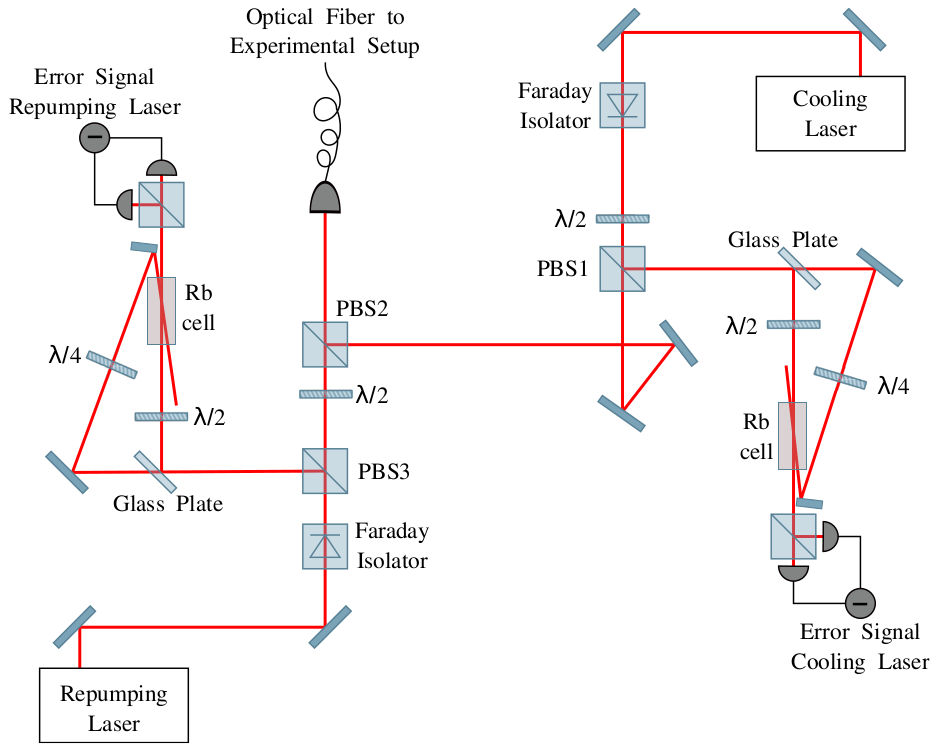
\includegraphics[width=0.5\textwidth]{figures/setup_laser.png}
  \caption{Setup of the pump laser and the cooling laser.}
  \label{fig:setup_laser}
\end{figure}

With an optical fibre the two beams get to the actual setup of the MOT which can be seen in figure \ref{fig:setup_mot}.

\begin{figure}[h]
  \centering
  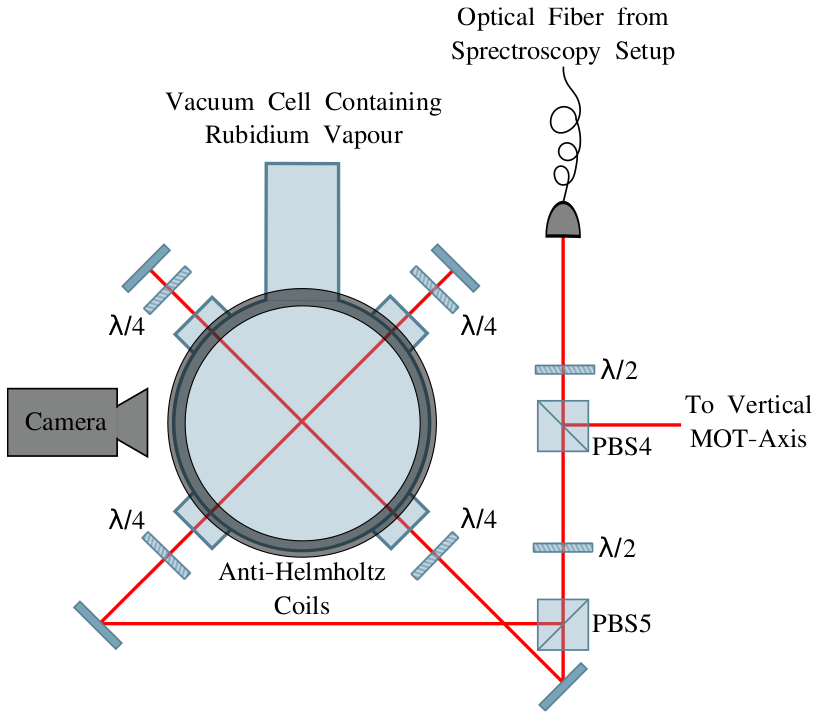
\includegraphics[width=0.5\textwidth]{figures/setup_mot.png}
  \caption{Alignment of the lasers in the MOT.}
  \label{fig:setup_mot}
\end{figure}

\subsection{Adjustment of the Beams}
As a first step we adjust the alignment of the beams in figure \ref{fig:setup_mot}. It is important that the beams cross each other in the center of the quadrupole field. This can be checked with the camera es the tutor showed us where the beams should cross each other on the display. With a CCD-camera\footnote{With the camera we can see the fluorescence of the rubidium atoms in the chamber.} we make sure that the beams really cross in one point. Using an aperture we make sure that each reflected beam is parallel to the original beam. A picture of the resulting setup can be seen in figure ???.\\ \\

???\\ \\

Additionally one must make sure that the power of the laser is split into three equal parts (for each axis). To do so we measure the power of each of the three beams with the powermeter. Adjusting the $\lambda/2$-plates we get an equal intensity of about \SI{1.2}{\milli\watt} per axis (in the original laser setup). This adjustment is done with the pumping laser turned of as we are only interested in the intensity of the cooling laser beeing equal for each axis. 
